\begin{filecontents}{bibtexlogo.sty}

\usepackage[utf8]{inputenc}
\usepackage{graphicx}
\usepackage{amsmath}
\usepackage{svg}
\graphicspath{ {./images/} }
\usepackage{helvet}
\usepackage{subcaption}
\usepackage{lipsum}
\def\lowBibTeX{{\reset@font\rmfamily B\kern-.05em%
    \raise.0ex\hbox{\scshape i\kern-.025em b}\kern-.08em%
    T\kern-.1667em\lower.7ex\hbox{E}\kern-.125emX}}
\def\BibTeX{\protect\lowBibTeX}
\end{filecontents}
%\documentclass[a4paper]{article}
\documentclass[12pt]{article}
\renewcommand{\contentsname}{Table of Contents}
\usepackage{harvard}
\usepackage{float}% If comment this, figure moves to Page 2
\usepackage{bibtexlogo}
	\addtolength{\oddsidemargin}{-.500in}
	\addtolength{\evensidemargin}{-.500in}
	\addtolength{\textwidth}{1in}
	\addtolength{\topmargin}{-.500in}
	\addtolength{\textheight}{1in}
\usepackage{helvet}
\newcommand{\comname}[1]{{\bf $\backslash$#1}}
\newcommand{\keyword}[1]{{\bf #1}}
\newcommand{\varname}[1]{{\em #1}}
\newcommand{\harvard}{{\sf harvard}}
\newcommand{\Harvard}{{\sf Harvard}}
\renewcommand{\familydefault}{\sfdefault}
\setlength{\parindent}{0em}
\setlength{\parskip}{1em}

\setlength{\arrayrulewidth}{1mm}
\setlength{\tabcolsep}{18pt}
\renewcommand{\arraystretch}{1.5}

%\usepackage{natbib}
\usepackage[version=4]{mhchem}
\begin{document}
\pagenumbering{gobble}
\begin{titlepage}
   \begin{center}
       %%%%%%%%%%%%%%%%%%%%%%%%%%%%%%%%%%%%%%%%%%%%%%%%%%%%%%%
       \large
        
\includegraphics[scale=0.4]{logo}
       \\
       \vspace{0.5cm}
        \textbf{SCHOOL OF ENGINEERING} \\

        \textbf{ENGG341 INDIVIDUAL PROJECT}
        
        
            
       \vspace{1.5cm}

 
       \vspace{1.5cm}
       \textbf{\Large{3D-printed Origami solar sails for Next Generation of CubeSats: Multi-body folding dynamics}}\\
       \normalsize
       
      \large{\textbf{Final Report}}\\
      
       \vspace{1cm}
      \Large{\textbf{Raymond Arturo Minarro Escalona}}\\
       \large{\textbf{BEng Aerospace Engineering\\May 2021}}\\
        \vspace{1cm}
      \Large{\textbf{Supervisor: Dr Stefania Soldini}}\\
      \large{\textbf{Project No. 201}}\\
      
      

       \vfill
        \textbf{
        \large
       School of Engineering
            \\
        University of Liverpool 
        \\
        Brownlow Hill, Liverpool, L69 3GH
        }
       \vspace{0.8cm}

       \normalsize
       %%%%%%%%%%%%%%%%%%%%%%%%%%%%%%%%%%%%%%%%%%%%%%%%%%%%%%%
   \end{center}
\end{titlepage}

\bibliographystyle{agsm}
%\bibliography{harvard.bib}
\section*{Summary}

CubeSats have become the go-to solution for affordable scientific experiments in deep-space, however, the disposable mass used as fuel for these CubeSats pose a significant weight constraint and lifetime expectation on the instruments on board. Solar sails seek to exploit solar radiation pressure to push the CubeSats in direction of the radiation without need for solid fuel. In this project, Python-based time-discrete numerical simulations were made to study the deployment of panels that form the sail, taking into account oscillations and variation of the solar constant. It was estimated for a triangle-based solar sail of area $43.3m^2$ thrust of $153.43\mu N$ is achievable at an orbit of height 1.5 AU (Martian orbit range), and over $790.8\mu N$ at an orbit of height 0.5 AU (Mercury orbit range).

%\lipsum[1]
\pagenumbering{gobble}

\pagebreak
\tableofcontents

\pagebreak
%%%%%%%%%%%%%%%%%%%%%%%%%%%%%%%%%%%%

\section*{Table of Notation}

\begin{tabular}{ p{1cm} p{10cm} p{5cm} }
\textbf{Symbol} & \textbf{Description} & \textbf{SI Units} \\

$\alpha$ & Angular acceleration of panel & $ rad \cdot s^{-2}$\\
$\gamma$ & Angle of sail away from Sun radiation direction & $rad $\\
$\delta$ & Difference over time-step & N/A \\
$\zeta $ & Damping ratio of dynamic system & N/A \\
$\theta$ & Angle of panel & $ rad $ \\
$\rho_{PLA}$ & Density of PLA printing filament & $Kg \cdot m^{-3}$ \\ 
$\omega$ & Angular velocity of panel & $ rad \cdot s^{-1} $\\
$\omega_n$ & Natural frequency of dynamic system & $ rads \cdot s^{-1} $ \\
$A_{panel}$ & Area of a panel & $m^2$ \\ 
$F_{SRP}$ & Force due to solar radiation pressure & $Kg \cdot m \cdot s^{-2}$ \\
$G_{SC}$ & Solar constant & $ Kg \cdot s^{-3}$ \\
$h$ & Height of panel & $m$ \\
$I$ & Moment of Inertia & $ Kg \cdot m^2$ \\
$l$ & Length of Panel & $m$ \\
$M_{spring}$ & Moment due to spring & $Kg \cdot m^2 \cdot s^{-2}$\\
$M_{SRP}$ & Moment due to solar radiation pressure, same as torque & $Kg \cdot m^{2} \cdot s^{-2}$ \\
$R_s$ & Radius of orbit around the Sun & AU \\
$T_p$ & Torque on panel & $Kg \cdot m^{2} \cdot s^{-2}$ \\
$c$ & Damper coefficient & $Kg \cdot m^2 \cdot s^{-1} \cdot rad^{-1}$ \\
$d$ & State of PDLCD & N/A \\
$k$ & Spring Constant & $ Kg \cdot m^{-2} \cdot s^{-2} \cdot rad$ \\
$p_{bus}$ & solar radiation pressure adjusted for bus distance from the Sun & $Kg \cdot s^{-2} \cdot m$ \\
$p_{SRP}$ & Solar radiation pressure & $Kg \cdot s^{-2} \cdot m$ \\
$t$ & Thickness of composite material & $m$ \\
\end{tabular}

\pagebreak


%%%%%%%%%%%%%%%%%%%%%%%%%%%%%%%%%%%%%%%%%%%%%%%%%%%%%%%

\pagenumbering{arabic}
\section{Introduction}

\subsection{Background}


\subsubsection{CubeSats}\label{CubeSats}


During the cold war, a race for technological development occurred between the United States and the late Soviet Union. This conflict gave way for the advent of deep-space scientific experimentation and data sampling. The use of artificial satellites, such as the 1957 \textit{Sputnik 1} proved the possibility of mounting scientific instruments on board bulky systems that may be inserted into quasi-stable orbits above the upper atmosphere. The \textit{Sputnik 1} was loaded with instrumentation that would make it possible to probe the ionosphere, sample the temperature and report it back to Earth via radio-frequency modulation \cite{Kuznetsov}.


% TODO: are one of these paragraphs the same?


After these historical successes on both nations, a new branch of scientific research was born: The making of artificial satellites that would provide answers and an overall better understanding of geophysics, astrophysics, research on climate change and even telecommunication. However, this was not affordable by many scientific agencies and were often constrained by on-board space, maintenance and economics. CubeSats became the ideal solution, providing low-cost access to upper-atmosphere and Low Earth orbit (LEO) sampling and instrument positioning for scientific and communication purposes thanks to its compact form factor, capability for bus mass-manufacturing and mass-launching. \cite{ExpCubesat}



\subsubsection{Propulsion systems}

As mentioned in previously, the standardisation of these small systems has opened the doors for the development of several propulsion systems for the small, purportedly lightweight satellites. Among those, there are chemical, electric, solid and propellant-less methods such as the solar sail 

In the chemical-based propulsion systems, a cold gas can be send outwards from the satellite to add momentum in one direction. The cold gas can be created from a high-pressure, compressed cold propellant in a canister, which poses threats of decompression and demands attention when designing the physical system willing to hold the pressurised material, adding to the fact that the satellite is already weight-constrained and designs often have small margins for propellant weight.

The electrical systems, such as electromagnetic or electrostatic field, plasma is generated from much less mass than the aforementioned chemical propulsion, and adds more momentum by accelerating the ions at a higher rate when disposed, effectively adding more momentum to the satellite at the cost of renewable energy such as electricity (when coupled with solar panels) on on-board batteries \cite{propulsion}.

As technology progressed, studies were made on the solar radiation pressure, which then prompted for new systems that utilise no on-board energy to produce thrust, but rather utilised only the solar energy available and rich in the outer space environment.

\subsubsection{Solar Radiation Pressure}\label{background:srp}


The sun is exists in a gravity-internal pressure equilibrium. It is composed mainly of hydrogen and helium, it creates the necessary energy to burn as hot through the nuclear fusion of Hydrogen into Helium (Eq. \ref{H}). Given that the products of the fusion are lighter than the starting Hydrogen, the release of electromagnetic quanta gives the sun the fuel necessary to burn hot and emits a black-body like radiation of 5700 K outwards and described as solar irradiance \cite{sunpower}.

\begin{equation}
%\ce{Na2SO4 ->[H2O] Na+ + SO4^2-}
%\ce{^{227}_{90}Th+}
\ce{4 ^{1}H -> ^{4}He + energy}
\label{H}
\end{equation}

Solar irradiance in itself is the total combined emissions perceived as coming from the sun. It has been studied extensively and measured throughout the spectrum of wavelengths (Fig. \ref{fig:background_spectrum}) that, when integrated it gives a flux density value described as the Total Solar Irradiance (TSI) which is defined and standardised as the solar constant. Due to the eccentricity of the Earth's orbit and the eventual appearance of sunspots, the true value of the solar constant oscillates. Averaged over a return period of 10-11 years (the Solar Cycle) and measured from space (e.g, no atmospheric losses), this value can be averaged and described as a flux density of $G_{SC} = 1.362 kW/m^2$ \cite{MagneticUniverse}

\begin{figure}[H]
\centering
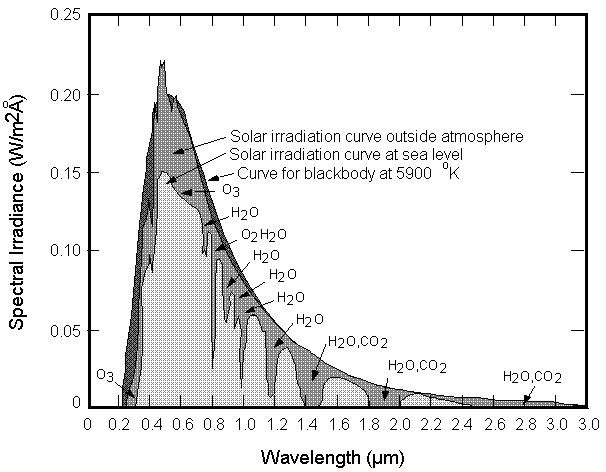
\includegraphics[width=0.75\textwidth]{images/spectrum.jpg}
\caption{Most of the solar irradiance energy comes from the visible light range and it is similar to that of a black-body radiation emission at 5700-5900 Kelvin \protect\cite{spectrum}}


\label{fig:background_spectrum}
\end{figure}




\subsubsection{Solar Sails}

A solar sail is any object that may deploy extensively around the satellite to cover a large area using the principles of solar radiation pressure. Such an area could attract significant thrust as a result of solar irradiance.

In the year 2010, the Japan Aerospace Exploration Agency (JAXA) launched its demonstration mission IKAROS (\textit{Interplanetary Kite-craft Accelerated by Radiation of the Sun})
which employed a 200$m^2$ sail and the pressure of the solar radiation to propel itself \cite{TakaoY}. This probe employed the method
described above to deploy its sail wherein the probe, cylindrical in shape, spun up and slowly unfolded the sail pinned to the sides of the
main body as depicted in Figure \ref{fig:deployment} \cite{pressIKAROS}. The purpose of this mission was to test the unfurling technology, including the steerability
of the vessel (attitude control) by changing the reflectance at points using polymer-dispersed liquid crystal devices (PDLCD) \cite{Ishida2016PolarizationEO}. However further
improvements to the storage and deployment methods are necessary if the size of the sail is to be increased as envisaged in the future mission to trojan asteroids named as OKEANOS \cite{TakaoY}.

\begin{center}
\begin{figure}
    \centering
    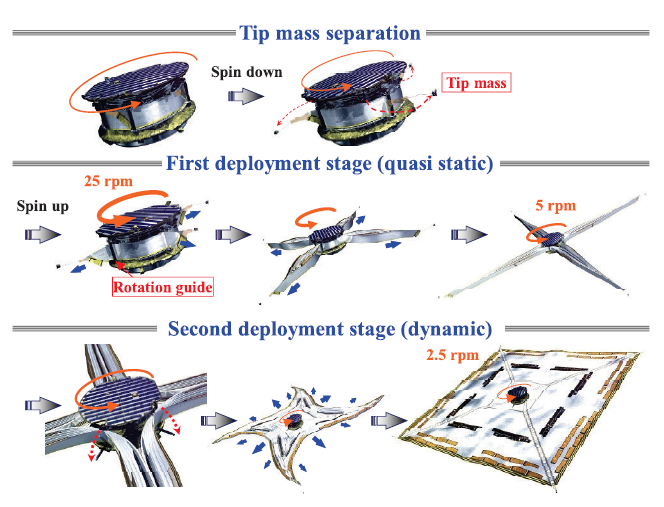
\includegraphics[width=100mm]{deployment}
  \caption{Deployment of Sail in the IKAROS mission \protect\cite{TakaoY}}
  \label{fig:deployment}
\end{figure}
\end{center}


One commonly used mechanism for storage methods of these sails is large, origami-like folding patterns of membrane/foil sails so as to
occupy as little space as possible when not deployed (Figure \ref{fig:origami}). Through many origami styles and projects, this objective is
achieved in smaller, recreational scales \cite{ZirbelS}.


\begin{center}
\begin{figure}[!htb]
    \centering
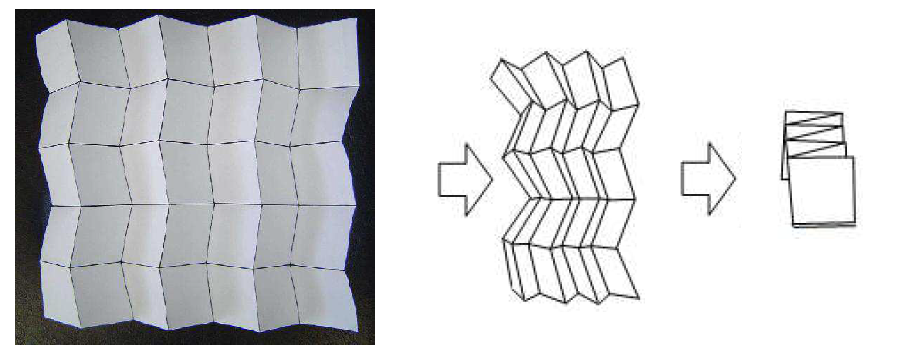
\includegraphics[width=0.9\linewidth]{origami2} 

\caption{Through origami, radial expansion from a packed, compressed thin membrane is possible, achieving satisfactory size ratios for CubeSats sail packing \protect\cite{Yutaka} }
  \normalsize
  \label{fig:origami}
\end{figure}
\end{center}



\subsubsection{3D Printing in Innovation}

In the recent years, 3D Printing technology has become widely utilised across many disciplines. From mechanical engineering companies practicing rapid prototyping within the day to issue a design proposal and test, to drug companies investing and investigating new ways of bringing drug delivery at a reduced cost. 3D Printing was welcomed industry users as it became an easy option to carry out vertical integration in supply chains. Users that were once required to obtain prototypes and specific part products, have now found a way to manufacture these requirements in-house. These can be printed at a reduced cost, increased speed and with relative easiness \cite{future3D}.

Furthermore, the advent of the information technology era has proliferated the ideas and knowledge of open hardware communities and organisations, the knowledge of these techniques is shared over mediums such as the internet and, being easily and readily accessible, have inspired users with industrial and domestic goals to adopt such technology and expand their skill set along with the capabilities of rapid prototyping and in-house polymer part manufacturing.


3D printing is a new technology that is friendly for inexperienced users and professional manufacturing plants and labs alike. Thanks to the cost savings, easiness of use and density of material that can be used, it becomes a strong candidate for affordable CubeSat part development, providing the strength and density necessary to carry out tasks in outer space.



\subsubsection{Numerical Simulation Fundamentals}\label{background:sim}

A simulation was made in Python utilising libraries like SymPy and Numpy, which allows the use of virtual inertial references frames for the sun, bus and panel components (Figure \ref{fig:sim_frames}). These panels may experience rotation and translation with respect to each other during the simulation. Thanks to SymPy's preferred "symbolical" nature rather than purely numerical, the coordinates and orientations of frames can be tracked with history and algebraic operations can be automatically called to prevent issues like the gimbal-lock, which is a prominent issue in simulations of this nature.


\begin{figure}[!htb]
\centering
\begin{subfigure}{0.5\textwidth}
  \centering
  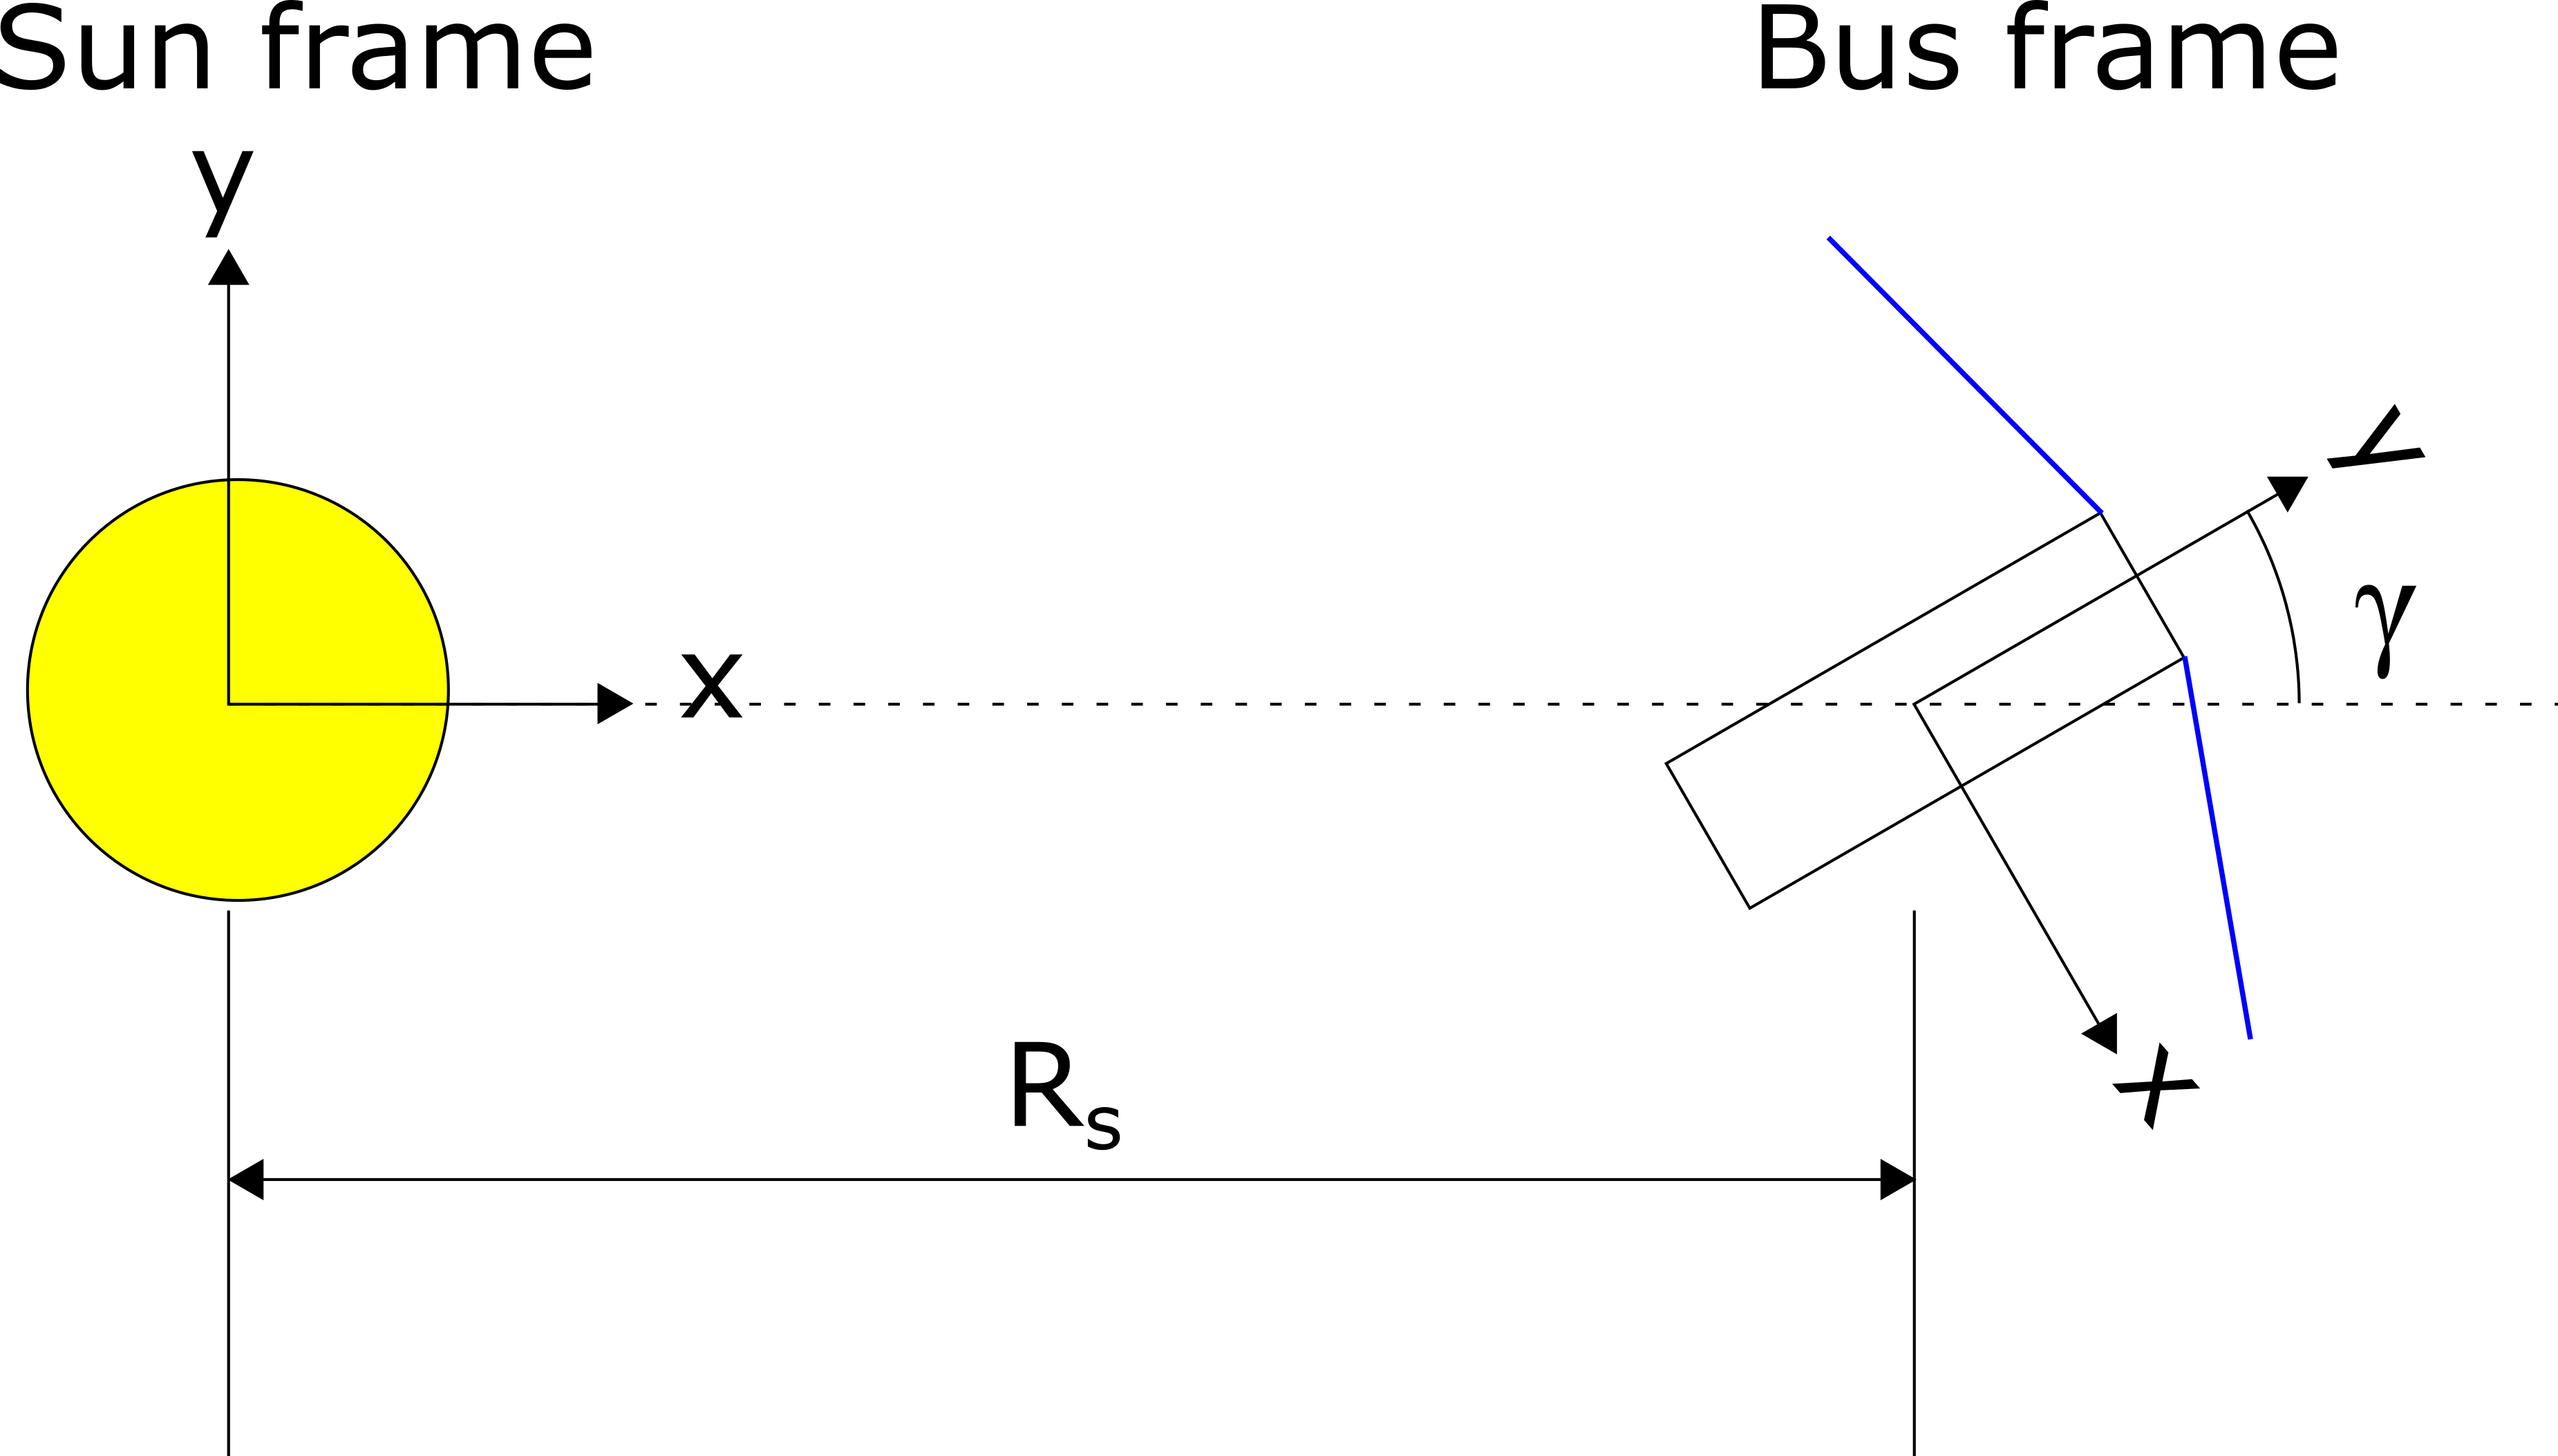
\includegraphics[width=0.7\linewidth]{images/sun bus frames.png}
\end{subfigure}%
\begin{subfigure}{.5\textwidth}
  \centering
  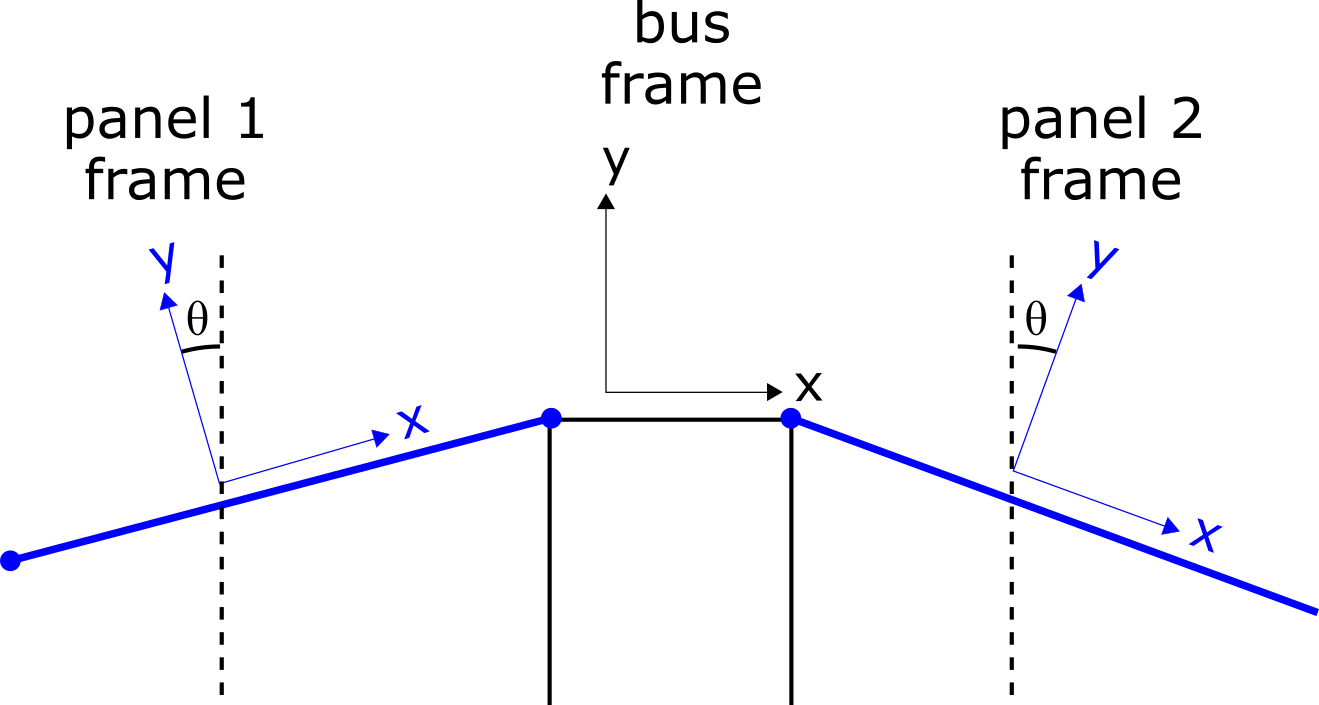
\includegraphics[width=0.7\linewidth]{images/bus panel frames.png}
\end{subfigure}
\caption{Reference frames within the simulation. Blue elements are panels (fully reflecting, $d = 1$) and black elements represent the bus of the CubeSat.}
\label{fig:sim_frames}
\end{figure}

In the discipline of physics and mechanic numerical simulations, there exists different methodology and basis by which different types of simulations arrive to a solution, or report lack thereof.

Different methods use different amount of computational resources and have different solving times depending on the complexity of the problem \protect\cite{simulations}. For the routine herein, a time-discrete state-space continuous is used:

\begin{itemize}
    \item \textbf{Time discrete}: The simulation begins at an initial state, which may be configured using the variables defined in \ref{experimental}. The variables are refreshed every time-step and handled accordingly. The process is repeated until a desired variable converges, e.g the number of significant figures desired do not change anymore between time-steps, and any further step taken only increases the precision (not necessarily accuracy).
    \item \textbf{State-space continuous}: The variables calculated therein fall within the spectrum of values that the simulation range is working with, yielding more precise values.
\end{itemize}

\subsection{Aim}

\subsubsection{Scope}

This project seeks to simulate a CubeSat solar sail being deployed. The simulation only dealt with projected surfaces normal to the sun and the values of solar constant $G_SC$ calculated at a pre-configured distance from the Sun. The simulation takes into consideration the reflectivity of each panel, representing the real-life state of the PDLCD devices, which can be edited as means of a 0 or 1 $d$ variable, the latter making the momentum obtained by reflection twice as high.

It does not take bending forces into account, which would be close to the real-life scenario where the bending forces could be negligible.

The simulation only indicated the time elapsed until a convergence is reached, along with plotting the angles for each panel throughout simulation time.



\subsubsection{Objectives}

The purpose of the project is to deploy a set of connected, 3D printed panels that convert into a sail large enough to impulse the vessel in a direction normal to the 
sun. In this report, a Python program has been under development to study the speed, damping and restive behaviour of the panels when extended by the solar radiation pressure. This will later on evolve onto a more complex simulation with the aim of studying the folding dynamics of a 3D printable sail. A set of aims are:

\begin{itemize}
    \item To study the multi-body dynamic behaviour of the deploying panels.
    \item To study the feasibility of more arrangements of unfolding panels to be used in the final design.
    \item To understand the physical principles governing the attitude control and impulse of the CubeSat in deep space missions.
    \item To study the efficacy of using SRP as source of impulse in deep space without the need for fuel.
    \item To suggest, based on the tests made, where the proposed solar sail could be most efficient in space missions.
\end{itemize}

\subsubsection{Deliverables}

The expected outcomes to this project are:

\begin{itemize}
    \item A Python-based numerical simulation code for the analysis of solid panels connected to a bus, being pushed by solar radiation pressure in a micro-gravity environment.
    \item A potential design for a triangle-based panel system that could be use as an initial proof of concept for a 3D printed solar sail.
    \item A published codebase available in BitBucket.
\end{itemize}


\subsection{Experimental project approach and methods}\label{experimental}



\subsubsection{Physics}

In order for motion to be calculated, the system was assumed to be a set of cantilevered panels connected to a central hub, which is either protruding out (in the case of a parallelogram CubeSat) or simply non-existent or not modelled. The volume of the CubeSat bus only dictates how shadows are cast on the panels, which is outside of the scope for this simulation.

In this problem, common rotational physical principles are used to rotate reference frames assigned to the different panels and the bus of the CubeSat. The dynamic system after which the simulation is modelled is iterated on and described in each type of simulation below.

During the first set of experiments, the panels were assumed to be rectangular and the bus to be a prism. The panels were connected through a flexible joint to both sides asymmetrically.

The bus is defined as a prism by common expected dimensions of 0.43m by 0.93m by 0.43m (width, length and depth respectively.) and a panel dimensions of length $l=0.7m$ and height of $h=0.7m$. This was done to test the effects of the simulated solar radiation pressure on the panels and what kind of behaviour to expect, and what additions would be made for the following tests.

The panel is assumed to be similar to high-end domestic polyactic acid (PLA) 3D printed layers of $50\mu m$. 3D PLA printers work by heating up PLA filament and setting it on a work surface close to each other to cool and form a solid, layered shape (Fig. \ref{fig:layers}). For a PLA filament of $\rho_{PLA} = 1.24g/cm^3$ \protect\cite{pladensity} then the panel will have an area-density according to Eq. \ref{density}

\begin{center}
\begin{figure}[!htb]
    \centering
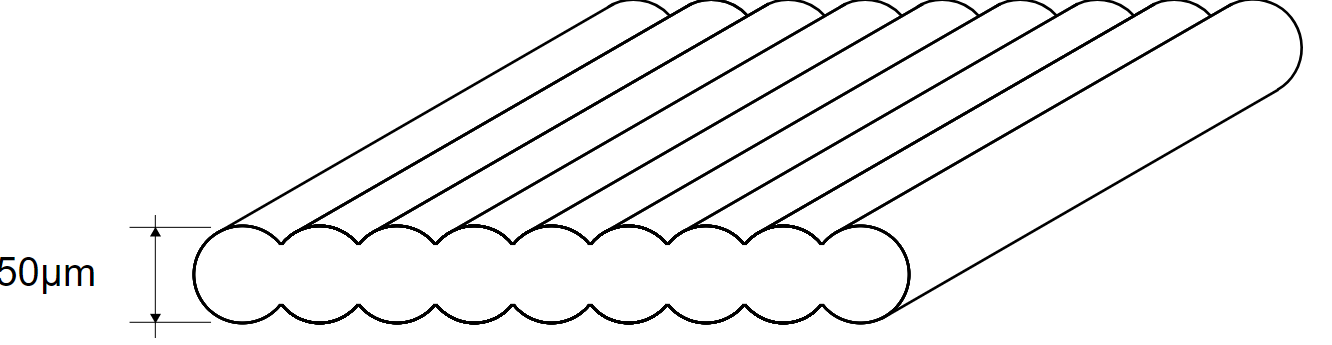
\includegraphics[width=0.7\linewidth]{layers.png} 
\caption{Assumed 3D printed layers made of tubular-like print traces with an average thickness of $50\mu m$}
  \normalsize
  \label{fig:layers}
\end{figure}
\end{center}

\begin{equation}
\rho_{A_{PLA}} = \rho_{PLA} t = 1240 kg/m^3 \cdot 50 \cdot 10^{-6} m = 0.062 kg/m^2 \label{density}
\end{equation}

In order to calculate moments of inertia to be used for rotation calculation, the general principle in Eq. \ref{MOI} is converted into a discrete-based operation in Eq. \ref{discreteMOI} which was then used for complex shapes and connection points.

In order to calculate the dynamical response per-time-step, the motion may be modelled after classic Newtonian physics (Eq. \ref{translation}) and the Euler equation \ref{rotation} applied to the cantilever systems depicted in Figure \ref{springSys}. It is worth noting that initially the velocity dampers $c\dot{x}$ and $c\dot{\theta}$ were not taken into consideration in \ref{res:squarepanelsconcentricarrangement}.

\begin{center}
\begin{figure}[!htb]
    \centering
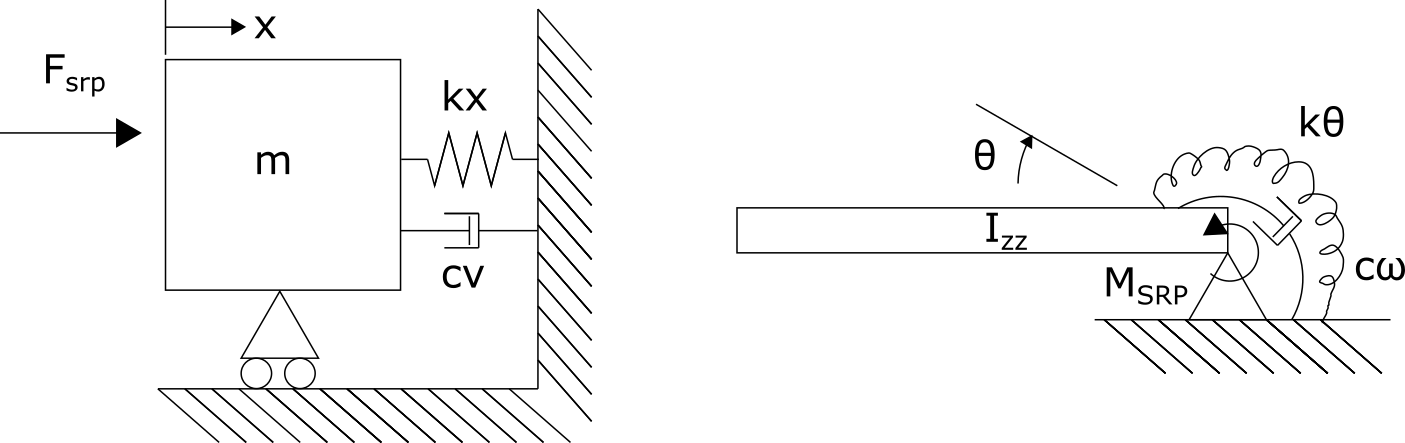
\includegraphics[width=0.7\linewidth]{images/spring damp system.png} 
\caption{Dynamic system assumed to study the behaviour of hinge moments between panels and the CubeSat bus.}
  \normalsize
  \label{springSys}
\end{figure}
\end{center}


\begin{equation}
    m\ddot{x} = F_{SRP} - kx - c\dot{x}
    \label{translation}
\end{equation}


and its rotational Euler equation:
\begin{equation}
    I_{zz} \ddot{\theta} = T_{SRP} - k\theta - c\dot{\theta}
    \label{rotation}
\end{equation}



For starting trials, the equation \ref{inertia} was derived for rectangular edge-connection example.

\begin{equation}
    I = \int_{0}^{M} r^2  \,dm
    \label{MOI}
\end{equation}

\begin{equation}
    I = \sum_{n=1}^{\infty} m_i \cdot r_i^2
    \label{discreteMOI}
\end{equation}

For a simple rectangle as described above, the equation may be simplified to equation \ref{inertia}.

\begin{equation}
    I_{zz}= \frac{1}{3} m*l = \frac{1}{3} l^2h\rho_{A_{PLA}} = 7.09\cdot10^{-7} 
\label{inertia}
\end{equation}

As outlined in \ref{background:sim}, the simulations were carried out in discrete time jumps, and a continuous state-space system. Variables like $F_{srp}$ panel torque $T_{p}$, angular acceleration $\alpha_{p}$, angular speed $\omega_{p}$ were calculated each cycle or time-step of $3.6s$. The time-step was chosen as a compromise between solve time and simulation of the system with real-life values, which are slow-acting due to the nature of the solar radiation pressure.
Given the problem summary, the forces acting on a panel assimilate to how forces on a pin-ended beam would behave, adding a torsional spring $-k\theta$ that opposes the torque $T_{p}$ caused by the force $F_{srp}$. An analogue system using a mass $m$ being pushed by $F_{srp}$ against a spring $kx$ causing a displacement $x$ similar to Fig. \ref{springSys} was used and modelled.


\subsubsection{Solar Radiation Pressure} \label{experimental:srp}

Most of the energy that constitutes the solar constant $G_{SC}$ is located on the visible light part of the spectrum. This means objects that would normally reflect this light will absorb some of the light's momentum opposite to the incidence direction. As such, this energy flux may be described as pressure constant by dividing it by the speed of light $c$ (Eq. \ref{Gsc}) \cite{solarhandbook}.


\begin{equation}
p_{SRP} = G_{sc}/c = 4.54 \mu N/m^2
\label{Gsc}
\end{equation}


The solar constant is used in astrophysics to identify the
energy carried by photons and other electromagnetic radiation expelled from the sun, measured as
flux density at an average Earth-Sun distance nominated as an
astronomical unit (AU), 1 AU has a fixed value of $1.49\cdot10^{11}$ meters \protect\cite{Astro}.

Given that the energy is propagated radially as a sphere away from the sun, the energy decrease is inversely proportional to the distance. As such, the inverse square law is applied to Eq. \ref{Gsc} to find the equivalent pressure at a distance of $R_s$ (Eq. \ref{angledp}), multiplied by the cosine of the angle $\alpha$ between the sun frame and the bus frame \protect\cite{sundyn}.

The pressure on a theoretical flat zone, normal to the sun, reaches a value described in Eq. \ref{Gsc}.

The solar constant is used in astrophysics to identify the
energy carried by photos expelled from the sun, measured as
flux density at an average Earth-Sun distance nominated as an
astronomical unit (AU), 1 AU has a fixed value of $1.49\cdot10^{11}$ meters \cite{Astro}.

Given that the energy is propagated radially as a sphere away from the sun, the energy decrease is inversely proportional to the distance. As such, the inverse square law is applied to Eq. \ref{Gsc} to find the equivalent pressure at a distance of $R_s$ (Eq. \ref{angledp}), multiplied by the cosine of the angle $\gamma$ between the sun frame and the bus frame \protect\cite{sundyn}.

\begin{equation}
p_{bus} = \frac{p_{SRP}}{R_s^2} cos(\gamma) = \frac{G_{sc}}{c R_s^2} cos(\gamma)
\label{angledp}
\end{equation}

Afterwards, this equivalent pressure $p_{bus}$ may be translated into a force acting on each panel ("panel" frame of reference) which may be oriented initially at an angle $\theta$ away from the bus frame, in addition to a state-trigger variable $d$ to model the PDLCDs \protect\cite{attitudeAndres}, giving Eq. \ref{totalFsrp}.
\begin{equation}
F_{srp} = cos(\theta)p_{bus}A_{panel}(1+d) = \frac{G_{sc}}{c R_s} cos(\gamma)cos(\theta)A_{panel}(1+d)
\label{totalFsrp}
\end{equation}

At this point, from the force normal to the panel, further mechanical simulation values may be derived.


\subsubsection{Work programme}
\begin{itemize}
\item Project and Team Kick-off meeting
    \begin{itemize}
        \item Identification of tasks: Divide the project into workable groups.
        \item Meeting for task allocation: That way each task is unique, well-defined and non-overlapping.
        \item Git repository setup: Since there is an available base of code from which to begin simulations, acquire access to it and familiarise myself with the version-control system used by the researchers (Milestone).
        \item Writing of a proposal document
    \end{itemize}
\item Resource improvement and liaison
    \begin{itemize}
        \item Literature review.
        \item Principles studies and testing: Exercises and thought-experiments for which I can prepare and compare my code to.
        \item Available code review.
        \item Available code testing: Make use of simple mathematical models for validation.
        \item Liaison for design: Get up to speed with design decisions taken by the mission planning group, work around this or give input.
        \item Requirement gathering: What is needed to carry out the simulation, what features it should have, and whether there are special mathematical principles to apply in it.
        \item Code development.
        \item New code testing and debugging.
        \item Code clean-up.
        \item Code documentation.
        \item Produce Interim Project Report (Milestone).
    \end{itemize}
\item Design iteration and convergence
    \begin{itemize}
        \item New code trial against expected simulation results.
        \item Iterative design changes
        \item Model clean-up: Preparation for write-up and conclusion.
        \item Conclusive design meeting
    \end{itemize}
\item Project conclusion
    \begin{itemize}
        \item Writing report.
        \item Presentation (Milestone).
    \end{itemize}
\end{itemize}

A revised Gantt chart (attached as appendix \ref{gantt}) was made to show the progress through these items over time.

\section{Results}


\subsection{Square Panels with Concentric Arrangement}\label{res:squarepanelsconcentricarrangement}

After the simulation terminated due to the value of $\theta$ reaching 90 degrees as seen in Fig. \ref{fig:1_results}, at which point it would start clipping the bus or folding "backwards", it was seen that the panel was oscillating and never converged.

\begin{figure}[!htb]
\centering
\begin{subfigure}{0.5\textwidth}
  \centering
  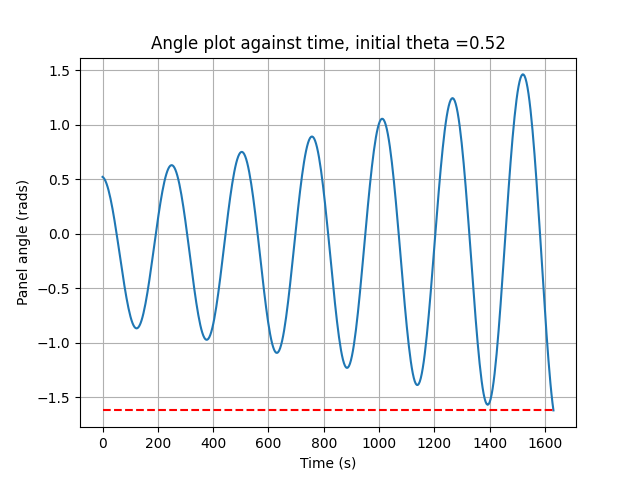
\includegraphics[width=1\linewidth]{images/first/theta_plot.png}
  \label{fig:1_theta}
\end{subfigure}%
\begin{subfigure}{.5\textwidth}
  \centering
  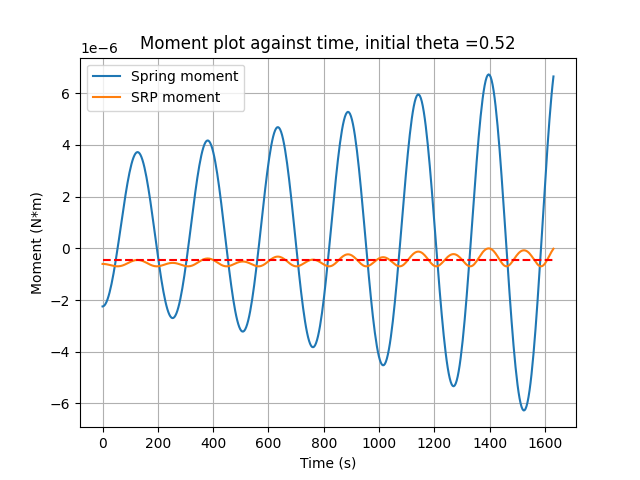
\includegraphics[width=1\linewidth]{images/first/moment_plot.png}
  \label{fig:1_moment}
\end{subfigure}
\caption{Simulation 1, the panel starts at a $\theta = 0.52 rads$ and does not converge.}
\label{fig:1_results}
\end{figure}



After further research, the initial system by which the simulation was mo\-del\-led represented a second-order dynamic system with a governing equation similar to a second-order ordinary differential equation:

\begin{equation}
f''(x) + af'(x) + bf(x) = u \label{dyneq}
\end{equation}
Where:
$$a = 2 \zeta \omega_n ; b = \omega_n^2$$

However, as there is not a $af'(x)$ factor, upon which depends the damping ratio $\zeta$, the present system would oscillate at a frequency of $\sqrt{k/I_{zz}}$

These results indicate that in real life, the system would need a mechanism to stop it from oscillating, be it a damper, or a system that counter-acts moment proportional to angular speed $\omega$ or $\dot{\theta}$. The reason why the amplitude of the oscillation increases is related to the limited minimum amount the system can accelerate every time-step, a smaller time-step would yield a system oscillating at a fixed amplitude.

Alternatively such a solution may be achieved by a electrically-controlled spring, which may activate/deactivate at its full spring coefficient $k$ frequently enough to maintain a neutral angular speed and therefore facing angle.

\subsubsection{Controllable spring simulation}\label{res:controlspring}

Instead of the spring being active permanently, an exception to the simulation may be added in such way that a closed-loop system activates the spring and applies counter-torque only when the angular acceleration of the panel $\alpha$ is above a certain negative threshold and the panel angle is close to the configured (Fig. \ref{numberline}).

\begin{figure}[!htb]
\centering
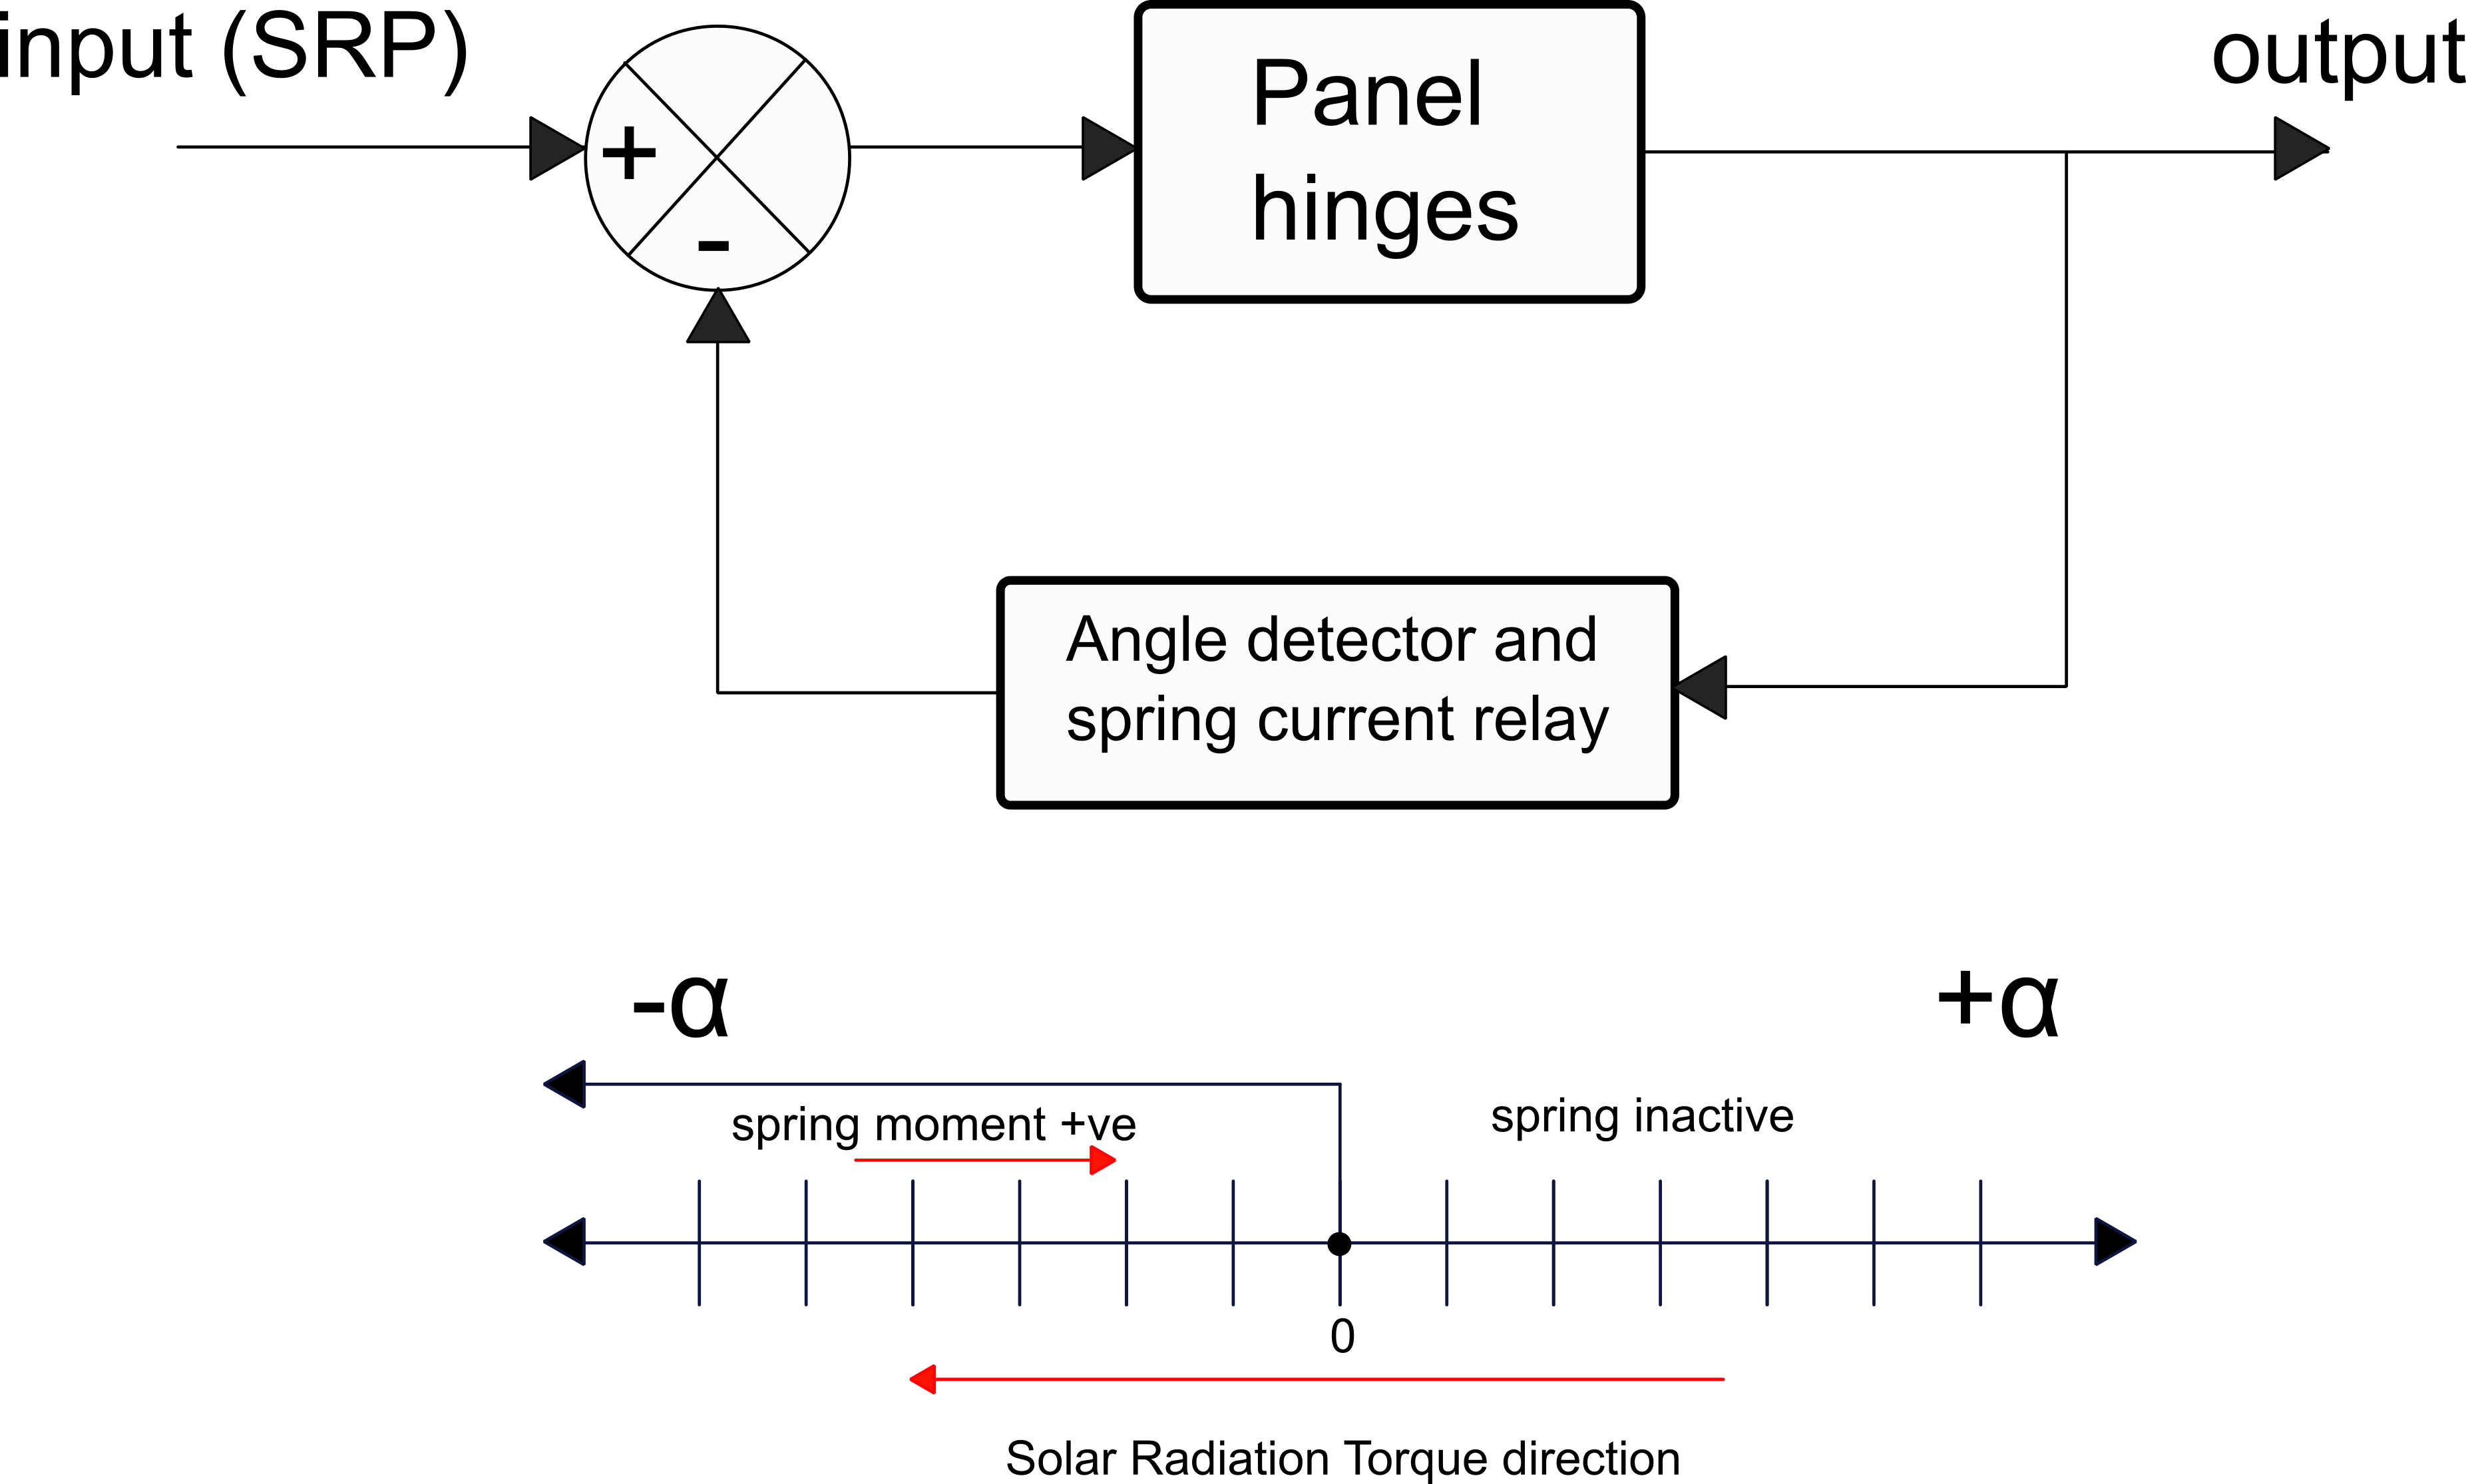
\includegraphics[width=1\textwidth]{images/clsystem.png}
\caption{"Approximate" converged diagram for Simulation 2. The panels oscillate close to a value of $\theta = 0$ where $F_{srp}$ is the greatest.}
\label{numberline}
\end{figure}

\begin{figure}[!htb]
\centering
\begin{subfigure}{0.5\textwidth}
  \centering
  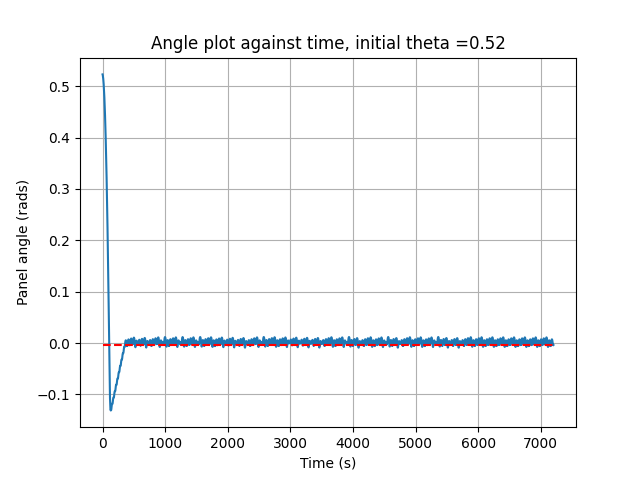
\includegraphics[width=1\linewidth]{images/second/theta_plot.png}
\end{subfigure}%
\begin{subfigure}{.5\textwidth}
  \centering
  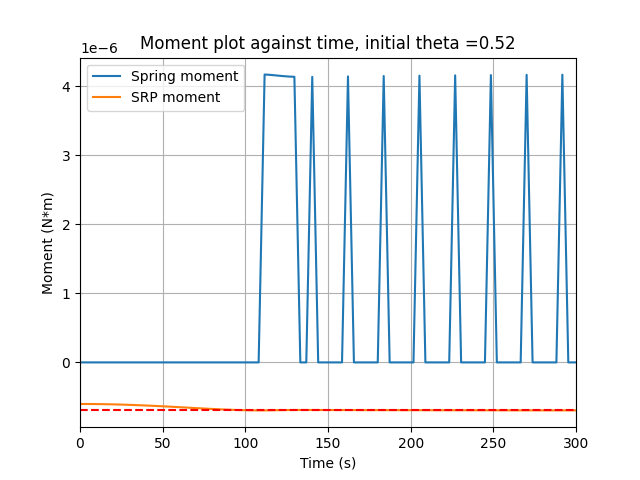
\includegraphics[width=1\linewidth]{images/second/moment_plot.png}
\end{subfigure}
\caption{Simulation 2 where in the spring is electrically activated which resulted in a small converged value around which $\theta$ oscillates.}
\label{fig:2_results}
\end{figure}


This means that when $\alpha$ is negative (accelerating forward towards the sail facing direction), the spring activates and delivers a moment (Eq. \ref{moment spring}), as it can be seen in Figure \ref{fig:2_results}.

   $$\alpha < 0 \implies k = k_{s}  $$
    $$\alpha \geq 0 \implies k = 0$$


\begin{equation}
    M_{spring} = -k(\theta - \theta_{ref}) \label{moment spring}
\end{equation}

\begin{figure}[!htb]
\centering
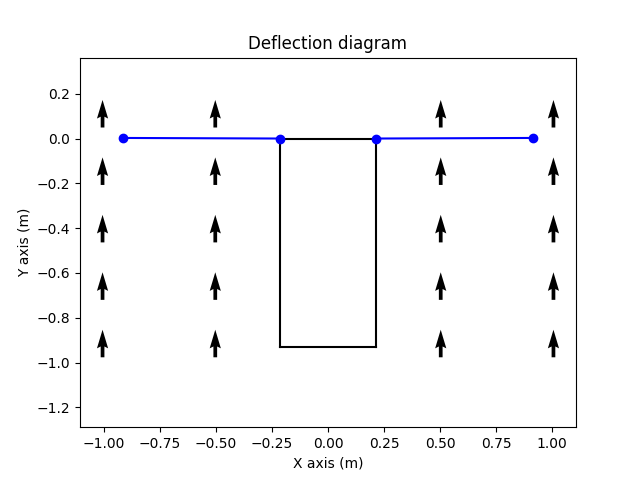
\includegraphics[width=0.5\textwidth]{images/second/deflection_diagram.png}
\caption{"Approximate" converged diagram for Simulation 2. The panels oscillate close to a value of $\theta = 0$ where $F_{srp}$ is the greatest.}
\label{fig:2_diagram}
\end{figure}


It is worth noting that due to $M_{spring}$ being far larger in magnitude than $T_{p}$, a single time-step is enough to cause a $\delta\alpha$ larger than the negative value of $\alpha$ that triggered the spring, driving the panel at a uniform pace until an angle of $\theta = 0$ is reached (See final "approximate" state in Figure \ref{fig:2_diagram}. This will yield a spring moment of 0 when triggered, self-balancing the system in a constant, small oscillation proportional to the time-step of the simulation.

This resulted on a system that oscillates around the converged value for $\theta$, as with the first simulation, the amplitude of the post-convergence oscillation is proportional to the minimum amount of acceleration in one time-step. In this particular example, the time for convergence was about 300 seconds for radial orbit of 1.5 AU, the panel rotated from an initial state of 30 degrees or 0.52 radians. Here "convergence" is defined as the point at which the dynamical behaviour of angle of the panel became cyclical, predictable and averaged to 0 degrees over time.

Due to the sensitivity of the system triggering the spring after the threshold, the panel never became static and reached angles between 0.01 and -0.008 radians (Fig. \ref{tinyoscillations}), which reduces the total $F_{SRP}$ averaged over time slightly.

\begin{figure}[H]
\centering
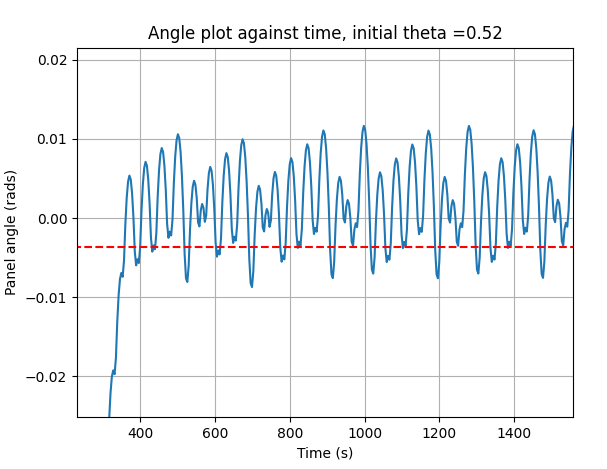
\includegraphics[width=0.8\textwidth]{images/second/tinyoscillations.png}
\caption{Zoomed-In Fig. \ref{fig:2_results} After "convergence" the panel oscillated a small amount while the spring turned on and off in accordance to the threshold.}
\label{tinyoscillations}
\end{figure}

\subsubsection{Passively damped simulation}\label{res:pasdamp}

Following the suggestions of adding a damping mechanism to comply with the dynamic equation \ref{dyneq} describing a second-order system, an arbitrary value of $\zeta = 0.45$ is chosen for the new system (Figure \ref{fig:3_system}), and the simulation tweaked to take this into consideration.

%The new dynamical system equivalent (Figure \ref{fig:dampspring} %has a damper with coefficient adjusted to achieve the $\zeta$ %value desired.

%\begin{figure}[h]
%\centering
%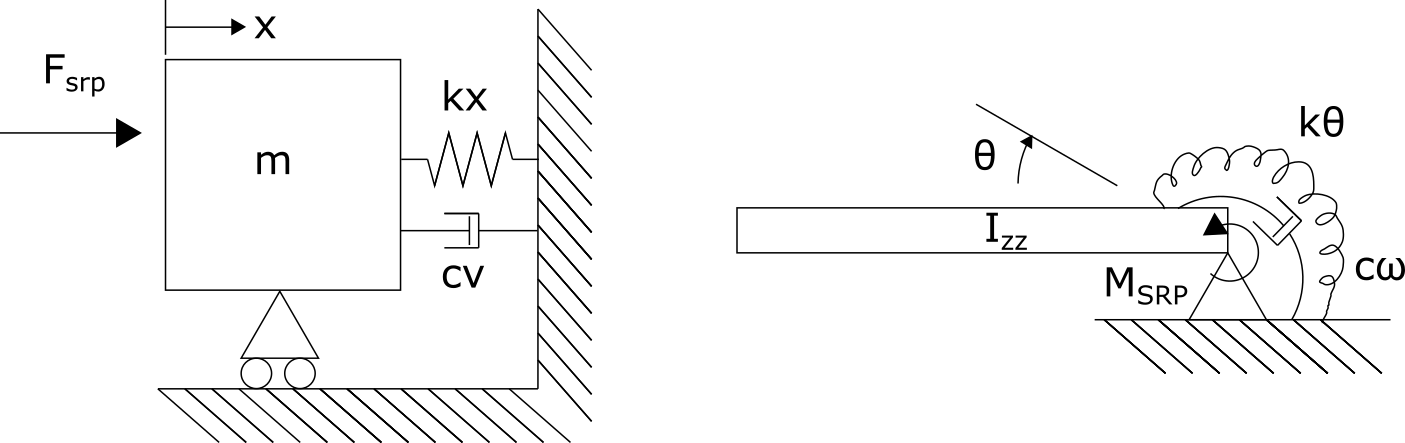
\includegraphics[width=\textwidth]{images/spring damp system.png}
%\caption{New equivalent dampened dynamic configuration} %\label{fig:dampspring}
%\end{figure}
%

\begin{figure}[!htb]
\centering
\begin{subfigure}{0.5\textwidth}
  \centering
  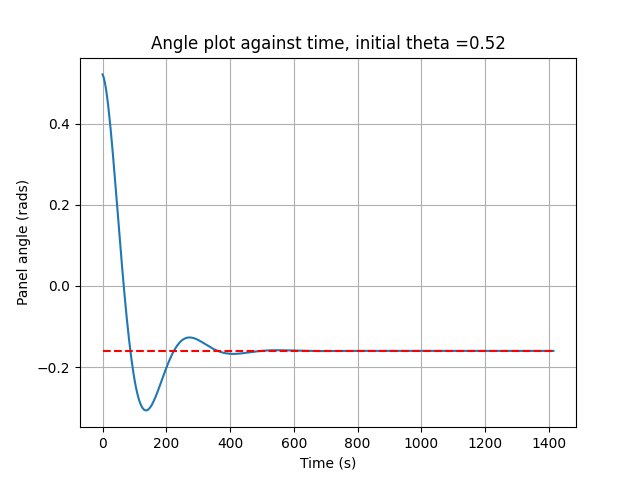
\includegraphics[width=1\linewidth]{images/third/theta_plot.png}
  \label{fig:3_theta}
\end{subfigure}%
\begin{subfigure}{.5\textwidth}
  \centering
  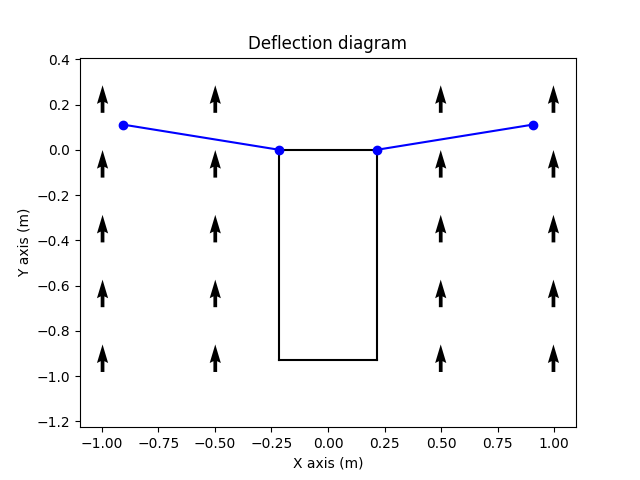
\includegraphics[width=1\linewidth]{images/third/deflection_diagram.png}
  \label{fig:3_deflection}
\end{subfigure}
\caption{Passive damping of $\omega$, the spring behaviour yielded an offset angle.}
\label{fig:3_results}
\end{figure}

As shown in Fig. \ref{fig:3_results}, the starting angle was the same as the previous test at 30 degrees. The angle converged slower at 400 seconds due to the damping in the system being less effective than the electrical spring, yielding a precise offset angle of -9 degrees where the moment of the spring is balanced out by the torque of the panel. This offset decreases slightly the total force achievable as noted by the higher moment peak. The final state converges at a point where $M_{spring} = T_{p_n}$, yielding a lower value of $F_{srp}$ than simulation 2.

\begin{figure}[H]
\centering
  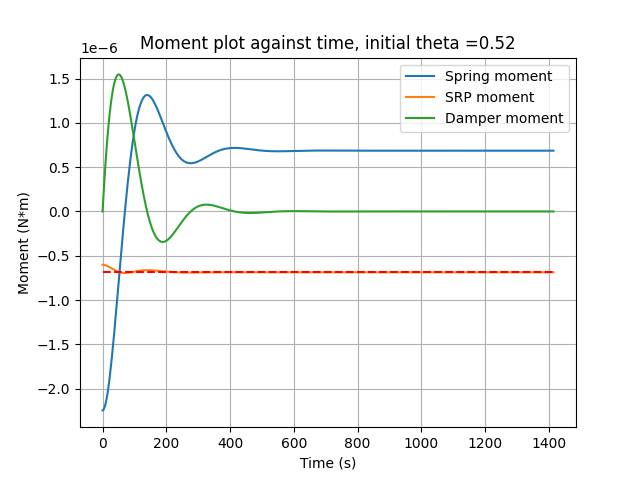
\includegraphics[width=0.7\linewidth]{images/third/moment_plot.png}
  \label{fig:3_moment}
\caption{Moments as calculated throughout the simulation, note the damper moment is eventually neutralised and the spring moment and the torque due to SRP are of equal magnitude and opposite signs, balancing each other out}
\label{fig:3_system}
\end{figure}

\subsection{Triangle Panels with Concentric Arrangement}\label{res:triangle}

In order to achieve a meaningful thrust force, the sails are arranged in a set of 3 connected radially to a triangular hub. Each panel now being 5 meters wide along the base. The damping is set to 0.45 and the spring coefficient $k$ to a sensible value of $9.5\cdot10^{-4} Nm/rad$.


As it can be seen in Fig. \ref{angletriangular}, the larger sails took around 500 seconds to settle and remain motionless. The final angle, like in the previous test, was an offset representative of the equilibrium between SRP and the string moment.

\begin{figure}[H]
\centering
  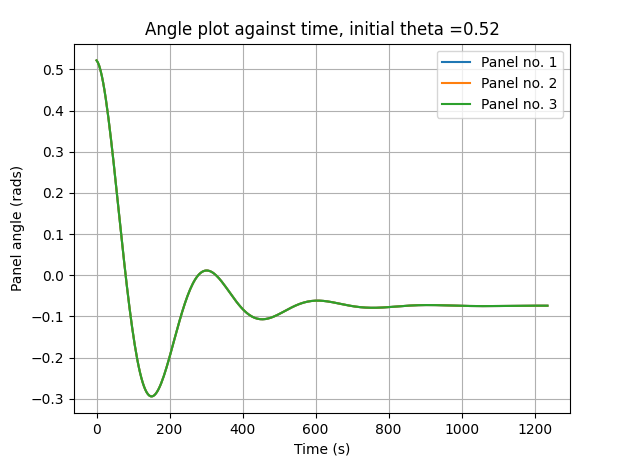
\includegraphics[width=0.7\linewidth]{images/third/forceconcentrictriangular.png}
\caption{Given that all the panels had the same state, they followed the same path and velocities when exposed to the same force.}
\label{angletriangular}
\end{figure}


\begin{figure}[H]
\centering
  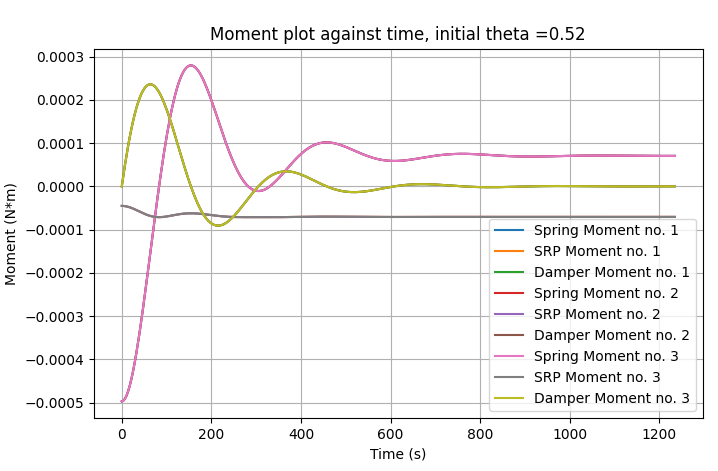
\includegraphics[width=0.7\linewidth]{images/third/momentconcentrictriangular.png}
  \label{momentconcentric}
\caption{The moments throughout the simulation. Note that there is only one line for Springs, one for Dampers and one for SRP given that all of them have the same value, they overlap each other perfectly in the graph.}
\end{figure}

\begin{figure}[H]
\centering
  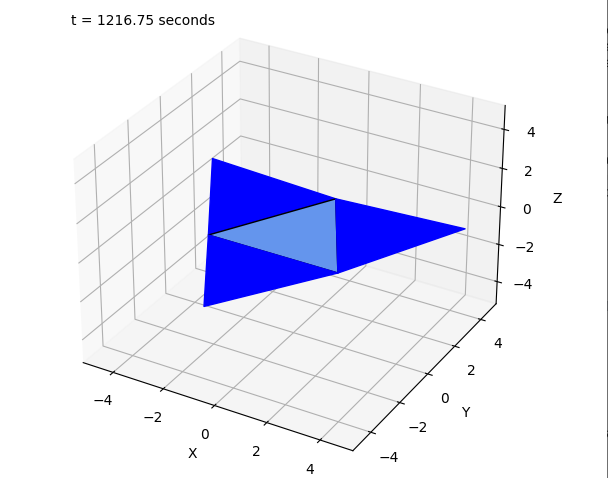
\includegraphics[width=0.7\linewidth]{images/third/concentrictriangular.png}
  \label{deployedtriangle}
\caption{Final state after convergence of the sail's panels.}
\end{figure}

At convergence, the thrust achieved by the sail's area was 153.43$\mu$N.

\subsection{Deployment from Compact Pyramid Shape}\label{res:pyramid}

When the panels are set to an angle $\theta$ of 120 degrees from their normal, a pyramid shape is achieved, with internal angles of 60 degrees as depicted in Fig. \ref{pyramid}.

\begin{figure}[H]
\centering
  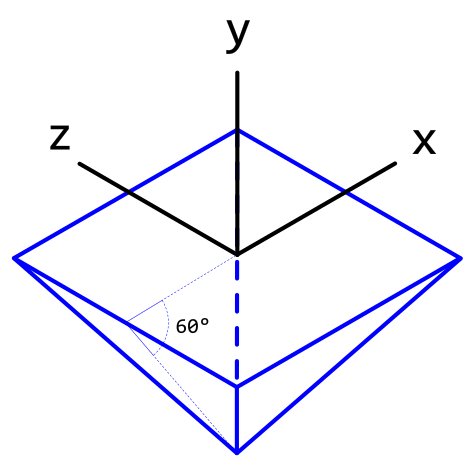
\includegraphics[width=0.5\linewidth]{images/third/pyramidshape.png}
\caption{Initial shape for the sail and inertial frame of references visualised.}
\label{pyramid}
\end{figure}

This resulted in the angle plot and moments plot in Fig. \ref{pyramidsim}, finally converging after 500 seconds into final shape in Fig. \ref{concentricsaildeployed}.

\begin{figure}[!htb]
\centering
\begin{subfigure}{0.3\textwidth}
  \centering
  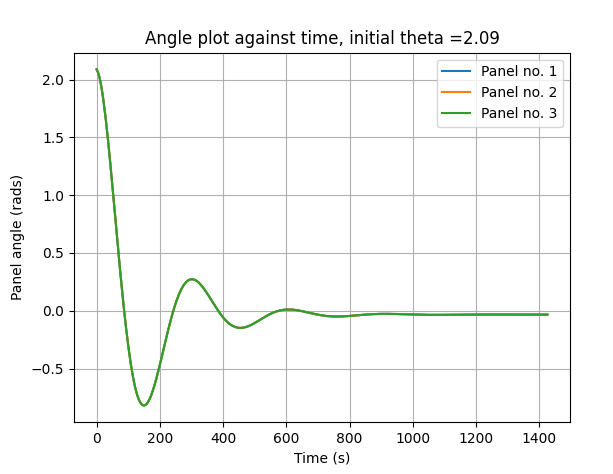
\includegraphics[width=1\linewidth]{images/third/angleconcentric pyramid.png}
\end{subfigure}%
\begin{subfigure}{.5\textwidth}
  \centering
  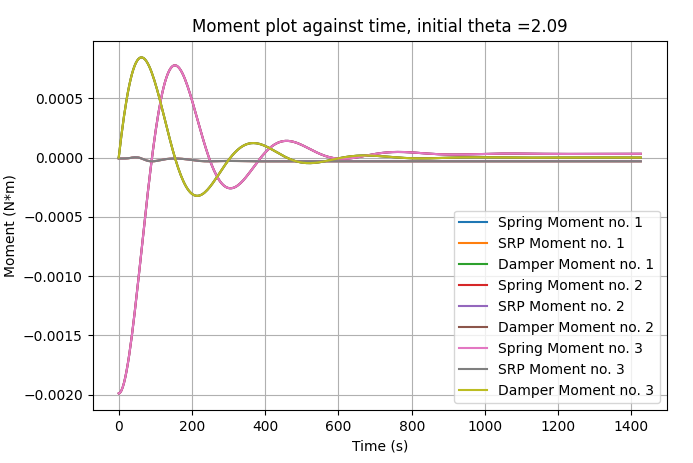
\includegraphics[width=1\linewidth]{images/third/momentconcentric pyramid.png}
\end{subfigure}
\caption{Passive damping of $\omega$, the spring behaviour yielded an offset angle.}
\label{pyramidsim}
\end{figure}

\begin{figure}[H]
\centering
  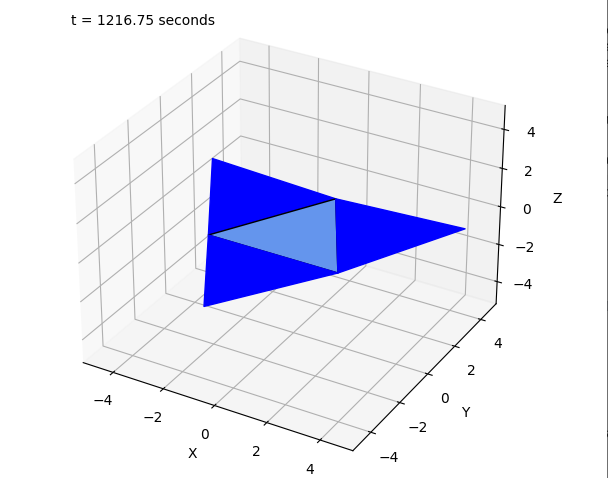
\includegraphics[width=0.5\linewidth]{images/third/concentrictriangular.png}
\caption{Final shape of the sail deployed.}
\label{concentricsaildeployed}
\end{figure}

In these settings, the force is 153.42 $\mu$Newtons of thrust.


\section{Conclusion}
\subsection{Discussion}

During test \ref{res:squarepanelsconcentricarrangement}, the first stages of the code were tested against small square panels attached to a dummy CubeSat bus. These panels yielded a negligible thrust due to their size and the fact that only two were tested in a 2D basis. It, however, provided great understanding on the effects of the solar constant $G_{SC}$ and how this one decreased exponentially the further away the sail is from the sun (Fig. \ref{gscplot}). It also provided a view into the necessity for a controlled spring mechanism, and/or damping. In reality, any system will have natural damping, however in outer space the number of molecules available to provide friction are much less and therefore the sail would rely on a natural damping inherited from the material it is made of.

\begin{figure}[H]
\centering
  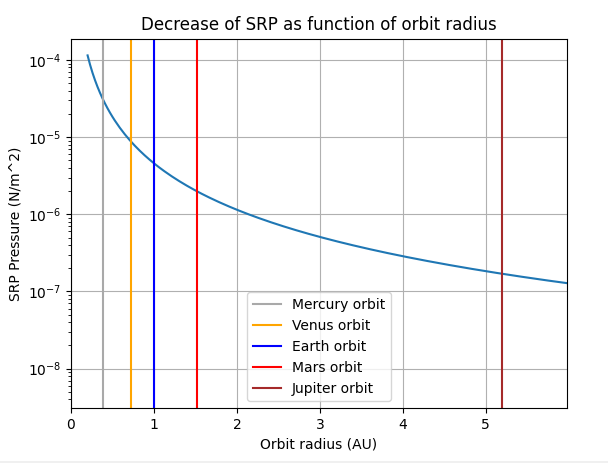
\includegraphics[width=0.75\linewidth]{images/pressuredecay.png}
\caption{Initial shape for the sail and inertial frame of references visualised.}
\label{gscplot}
\end{figure}

Continuing on to test \ref{res:controlspring}, great advances were made by designing a closed-loop system capable of triggering the now electrical spring mechanism, however it made the unrealistic assumption that the thermal action caused by current running through the spring is stable, immediate, and repeatably reliable. The suitability of this idea for the design is beyond the scope of this project, however it is worth mentioning that the system merits more investigation and testing to properly assess the suitability of the system. On test \ref{res:pasdamp}, the natural damping described above was taken into consideration with a value of $\zeta = 0.45$, yielding convergence times in the hundreds-of-seconds. This method was used as the basis for the following tests. At this height, the spring constant $k$ has been deduced to be $9.5 \cdot 10^{-6} NM/rad$, Given that the reference angle for the spring, $\theta_{ref}$ was set to 0 (assuming that the spring had a bias towards laying flat) in Eq. \ref{moment spring}, this means that for any balancing moment $M_{spring}$, there will have to be a non-zero $\theta$ which will provide the right compression/extension on the torsional spring to neutralise the torque $T_p$ caused by SRP. The weaker $k$, the higher the final offset angle will be.


At test \ref{res:triangle}, a triangle-shaped panel based 3D sail was designed, the whole system had a width of 10 meters at the base, giving an overall total area of around $43.3m^2$. The system oscillated between certain angles before settling down in the range of the 400-700 seconds.

Lastly, on test \ref{res:pyramid}, a initial state with an angle of 120 degrees (60 degrees internal) starts the sail compacted into a pyramid, which is then extended and stabilised at a point where the moments balanced out.

Both of these previous tests yielded a thrust of $153.42 \mu N$, thanks to the solar irradiance, and as discussed in \ref{background:srp}, the general thrust caused by a sail this size would be on the hundreds-of-micro-newtons magnitude, potentially reaching the milli-newton range at a distances below 0.5 AU from the sun, these orbits coincide with the mercurial orbits. Making the sail very useful at inner-planet reconnaissance missions. For comparison the IKAROS mission in Venus measured a thrust of $1.12mN$ \cite{TakaoY} at a Venus orbit with a radius of 0.72 AU. The average pressure felt by the IKAROS' solar sail, assuming that its plane is normal to the radiation direction is as shown in Eq. \ref{Ikarossrp}.

\begin{equation}\label{Ikarossrp}
    p_{SRP_{IKAROS}} = 1.12 \cdot 10^{-3} N / 200 m^2 = 5.6 \mu N
\end{equation}

This is comparable to the SRP estimated around Venus to be $8.8 \mu N$ (Following Eq. \ref{angledp}). This practical value $p_{SRP_{IKAROS}}$, being 36\% lower, deduces that the values estimated herein are probably too theoretical and omits several factors that may decrease efficiency, bending of panels, wrinkles and imperfection on the sails, the angle being far from normal to the direction of radiation, and so on. 

It is estimated that at an orbit height of 0.5 AU (Mercury orbit range), the total thrust achieved by the solar sail could be up to $790 \mu N$.

Further information regarding other solar sails projects was sought to no avail. The Planetary Society's LightSail 2 reported a success in LEO, however they also estimated that the mission would not be as lasting as other LEO CubeSat missions due to the sail posing a huge drag factor, and the density of the Earth's atmosphere still causing a considerable amount of aerobraking \cite{planetary}. This limits the recommendable use of the solar sail presented in this project to inner-planet orbits. Atmospheres like Venus' and Earth's are dense and pose a threat to the aerobraking capabilities of a large sail if the CubeSat is operated close to them, however thin exospheres like Mercury's are mostly harmless.

With this:

\begin{itemize}
    \item The multi-body dynamic behaviour of the system has been studied and described.
    \item The arrangement of the panels in a triangular shape is large enough to deliver significant thrust.
    \item The physical principles behind how the thrust is generated and its variation has been studied.
    \item SRP has demonstrated to be efficient in a theoretical way, and also practical by giving examples of numerical results expected.
    \item A mission specification has been suggested to for which the solar sail is most suitable, that is, inner planets non-atmospheric reconnaissance missions.
\end{itemize}

\subsection{Potential Improvement}
\subsubsection{Ray-tracing}

Currently, the simulation relies on the calculation of "equivalent-exposed" surface, taking into consideration the angle of the CubeSat (or bus) against the Sun, and the angle of each panel with respect to the bus. The system never took into consideration shadows cast by the bus or other panels, or considered rays that may have hit one panel and reflected in a way that reached the other. Situations like the compact pyramid deployment are estimated to have its panels move faster in real life as the EM radiation entering the pyramid after a few seconds would bounce several times between the panels before finally escaping, effectively losing more energy to the transferred momentum.

Several simulation technologies use ray-tracing to predict the bouncing of light on objects, and whether these bounced rays hit any other surfaces. Thanks to the technology available, this could be used to reduce the time the Python simulation spends calculating the equivalent exposed surfaces \cite{RayTracing}. Taking this into consideration may not only represent a more realistic scenario but also help study any improvement that could be made to exploit the reflection and entrapment of light to deploy sails faster.


\subsubsection{Dynamic Spring Constants}

For the previous simulations, a static value of the spring constant $k$ was used. If this spring was to be implemented in real life by means of a wiring running current and heating up, then further studies and investigation regarding the thermal dissipation of this wiring needs to be made. As it stands, this current must be sufficiently high to heat up the wire enough to transmit this thermo-elastic behaviour onto the solar sail it is mounted on, and the transmission of this may be harder to understand in an environment such as space, making real life in-atmosphere testing not nearly comparable or valid.


\pagebreak

\section{Bibliography}
\bibliography{harvard}
\pagebreak
\appendix
\pagebreak
\section{Gantt Chart} \label{gantt}

\end{document}
